\documentclass[tikz,border=10pt]{standalone}
    \usepackage{tikz}
    \usetikzlibrary{arrows.meta}
\begin{document}
	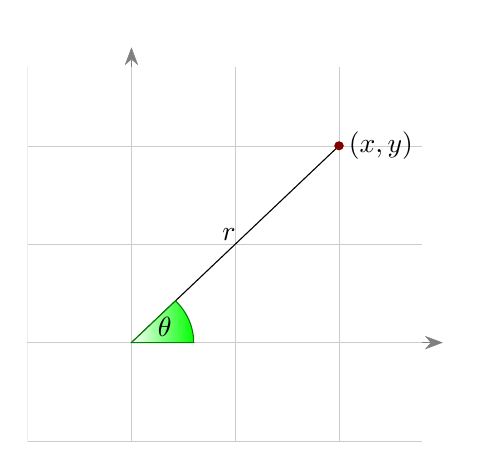
\begin{tikzpicture}[
 	         x                = 30,
	         scale            = 2.5,
             axis/.style      = {help lines, -{Stealth[length = 1.5ex]}}]
             \clip (-0.5,-0.5) rectangle (1.6,1.6);
             \draw [axis] (-1.5,0) -- (1.5,0);
             \draw [axis] (0,-1.5) -- (0,1.5);
             \draw [step=0.5,white!80!black,very thin] (-1.4,-1.4)
                    grid (1.4,1.4);
             \draw  (0,0) -- (1,1) node[anchor = west]{$(x,y)$} ;
             \filldraw [red!50!black] (1,1) circle [radius =0.02];
             \shadedraw[left color=white,right color=green, draw=green!50!black]
                   (0,0) -- (0.3,0)
                   arc [start angle=0, end angle=45, radius=0.3] -- cycle;
             \draw (0.16,0.08) node {$\theta$};
             \draw (0.47,0.55) node {$r$};
    \end{tikzpicture}
\end{document}
        